\documentclass[a4paper,kulak]{kulakarticle}

\usepackage[utf8]{inputenc}
\usepackage[dutch]{babel}
\usepackage[]{amsmath}
\usepackage{float}
\usepackage{subcaption}
\usepackage{graphicx,wrapfig,lipsum}

\date{Academiejaar 2018-2019}
\address{
  Informatica \\
  Statistische modellen en data-analyse \\
  Prof. Stefan Van Aelst \& Stijn Rebry}
\title{Verslag project 1}
\author{Thomas Bamelis \& Michiel Jonckheere}

\begin{document}

\maketitle

\tableofcontents
\newpage
\section*{Introductie}
\begin{wrapfigure}{r}{4cm}
	\caption{Mooiboi.}
	\label{fig:mooi}
	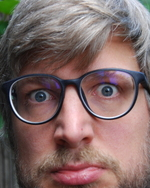
\includegraphics[width=4cm]{figures/stino.jpg}
\end{wrapfigure}
Dit is een zeer mooie man. \\
Zo mooi.\\
Zo geil. \\
Die blik.\\
Die lippen.\\
Wat als we van iedereen, wij, de prof en stino een afbeelding invoegen en deze van stino?

\section*{Besluit}


 
\end{document}
